% Chapter 3

\chapter{ Related work }
\label{Chapter3}
\lhead{Chapter 3. \emph{ Related work }}

\section{Über- and micro-shaders}

A popular solution to the shader permutation problem is the \emph{ über-shader }. In this approach, the programmer creates a large monolithic shader containing all the features a rendered object might need. Subsets of the functionality are then selected either at compile-time via preprocessor-based conditional compilation or at run-time via dynamic branching.

\begin{lstlisting}[frame=single]
#ifdef NORMAL_MAPPING
    float3 normal = sampleNormalMap(...);
#else
    float3 normal = normalize(interpolatedNormal);
#endif

float4 color = 0;
#ifdef DIFFUSE
    color += computeDiffuse(normal, ...);
#endif
#ifdef SPECULAR
    color += computeSpecular(normal, ...);
#endif
...
\end{lstlisting}

Über-shaders are conceptually simple and easy to implement, therefore work great with a low number of features. On the other hand, when the required number of achievable effects grows, über-shaders don't scale extraordinarily well. Since all features must be implemented within the same fragment of code, logic and data flow may become too complex to maintain and debug efficiently.

A more advanced take at the problem is to keep shader fragments separate and merge them conditionally using run-time logic or conservatively, yet statically generate permutations in the content pipeline. \citet{Hargreaves04} shows an approach based on runtime shader fragment combining. His implementation relies on a simple extension of the HLSL language in order to define the \emph{imports} and \emph{exports} of a shader fragment. Along with a special \emph{interface block}, a preprocessor is able to combine shader fragments together, linking their inputs and outputs. This effectively hides the complexity from the shader author, making maintenance and debugging easier. Hargreaves praises the robustness of this solution and mentions that it allows the usage of the same shader fragments in various rendering algorithms.

This work builds on shader fragment merging and extends it with automatic parameter type coercion and functional composition. I show how to implement such a scheme in a way that's easy to work with even for non-programmers.

% http://books.google.com/books?id=DgMSb_10l7IC&pg=PA555&lpg=PA555&dq=%22uber+shaders%22&source=bl&ots=-mu34jRtzO&sig=C3KIgqPIb6F8MDsOU0tSevVuN8M&hl=en&ei=zPZpTNGHNoGA4Aam1aHJCQ&sa=X&oi=book_result&ct=result&resnum=4&ved=0CCIQ6AEwAzgK#v=onepage&q=%22uber%20shaders%22&f=false

\section{RenderMan}

% TODO: the name is also a pun on Point Reyes

When designing a graphics rendering system, it is impossible not to bump into what currently constitutes the industry standard for film rendering -- RenderMan. Despite being over 20 years old, it continues to thrive as the benchmark for all rendering technology. It has been used in several dozen successful feature film productions and among its achievements is the first Oscar even awarded to the developers of a software package \cite{RenderManAwards}. An interesting aspect concerning RenderMan is that the overall structure of its Interface Specification (\emph{RISpec} in short) has survived mostly unchanged since its very first publication in 1988.

The rendering algorithm mainly utilized by Pixar's flagship implementation of RenderMan is called \textbf{REYES} (acronym for \emph{Renders Everything You Ever Saw}). It can be divided into the following steps:
	
\begin{enumerate}
\item \textbf{Bound} --- Conservatively cull off-screen objects using their bounding volumes. This early-out mechanism allows many calculations to be skipped for objects which can be trivially shown not to contribute to the final image.
\item \textbf{Split} --- Perform primitive-specific subdivision of the incoming geometry, generating more primitives as a result. Steps 1 -- 2 are evaluated recursively until the size of primitives meets a pre-configured threshold or a primitive declares that it is not splittable.
\item \textbf{Dice} --- Create a grid of \emph{micropolygons} from each primitive generated in the previous step. Each micropolygon is a quadrilateral approximately $^1/_2$ a pixel on a side. Micropolygons can be generated in a pattern matching the orientation of a texture applied to the primitive, enhancing quality via simplified filtering and improving performance due to access locality.
\item \textbf{Shade} --- Compute the lighting and shading at each vertex of the micropolygon grid.
\item \textbf{Sample} --- Generate the final image by stochastically sampling micropolygons for each pixel.
\end{enumerate}

It may seem that the algorithm is overly complex, especially when compared with regular rasterization, however it is able to exploit texture and geometric locality, parallelism and scales gracefully with increased scene complexity (\cite{Cook87reyes}). Stochastic sampling of micropolygons enables efficient computation of motion blur and depth of field effects. Finally, arbitrary primitive types are allowed, as long as they can be split or diced and finally converted into micropolygons.

The architecture is programmable via 5 \emph{shader} types (\cite{keyframeRSL1}):

\begin{description}
\item[Surface] --- Defines how a surface reacts to light, allowing the programmer to define its look. Surface shaders allow custom reflectance models to be defined, but also specify how the pigment or material of an object looks, hence allowing the definition of complete \emph{BRDF}s.
\item[Displacement] --- These shaders change the macro-structure of the surface, being able to alter normal vectors or offset the positions of micropolygons.
\item[Volume] --- Changes the color of light rays as they travel through a volume. May be used to create effects such as fog or smoke.
\item[Light] --- Represents the light source, allowing specification of light colors, shadows, intensity, falloff, ``barn door'' effects, etc. Computes the amount of lights which arrives at a particular point in space -- the surface being shaded.
\item[Imager] --- Imager shaders operate on image pixels just prior to the final output. They may be used e.g. to perform color correction or procedural background generation. Unfortunately, an imager shader being run for a single output pixel may only use the corresponding single pixel as an input, so more advanced effects, such as tone mapping (which require global or localized image statistics) are not feasible.
\end{description}

An important aspect of the RenderMan architecture is its ability to freely mix and match any primitives and shaders. Since every primitive eventually resolves to micropolygons, it can be used with any \emph{Displacement}, then processed by any \emph{Surface} shader. The latter may in turn interact with any \emph{Light} shaders, hence ensuring full orthogonality of the building blocks.

Unfortunately, micropolygon-based real-time rendering is still not viable for current commodity hardware. \citet{PatneyRealTimeReyes} present an implementation which performs the Bound, Split and Dice stages using NVidia CUDA, then passes the tessellated geometry into the regular OpenGL pipeline. While the tessellation stage achieves good performance, rendering the resulting micropolygons using conventional rasterization is suboptimal. Due to implementation details of current GPUs, there exists shading overhead for tiny polygons, with up to 8 times the theoretical cost for triangles spanning a single pixel \cite{understandingG80}.

Still, even without using micropolygon-based rendering, an architecture can be designed to retain some of the advantages RenderMan possesses. In particular, this thesis presents a shading framework decoupled from the shader domains imposed by current GPUs, instead moving closer to the model employed by RenderMan. Additionally, the limitation of \emph{Imager} shaders is lifted, hence enabling more sophisticated post-processing effects to be created.


\section{Deferred rendering}

The standard \emph{Forward} rasterization algorithm requires that material and light shaders for an objects be merged into a single GPU program. The implications are two-fold:
\begin{enumerate}
\item The lower bound on the number of GPU programs that need to be compiled is $O(m * l)$ (where $m$ stands for the number of materials and $l$ for the number of light shader \emph{combinations}), or \emph{multi-pass} rendering must be used.

The number of shaders created this way may be prohibitively large. One obvious workaround is to restrict the possible light shader combinations. This may be achieved via über-lights \cite{UberLights, UberLightsCg} or just constraining the renderer to a handful of light types. A related technique is to use a shader designed for more lights than what's necessary and zero-out any excessive light slots. For instance, when the renderer must render an object influenced by two point-lights, it may use a shader for rendering it with three point-lights, assuming zero intensity for one of the parameters. Naturally, this approach, just like the über-light one, carries a runtime cost which may be prohibitive in a complex setup.

An alternative solution to this issue is \emph{multi-pass} rendering, where the object is rendered once for an affecting light, and the resulting per-fragment irradiance is summed via additive blending. The downside is that in scenes with complex geometry, rendering objects multiple times will quickly drain the computational budget.

\begin{figure}[h!]
  \centering
    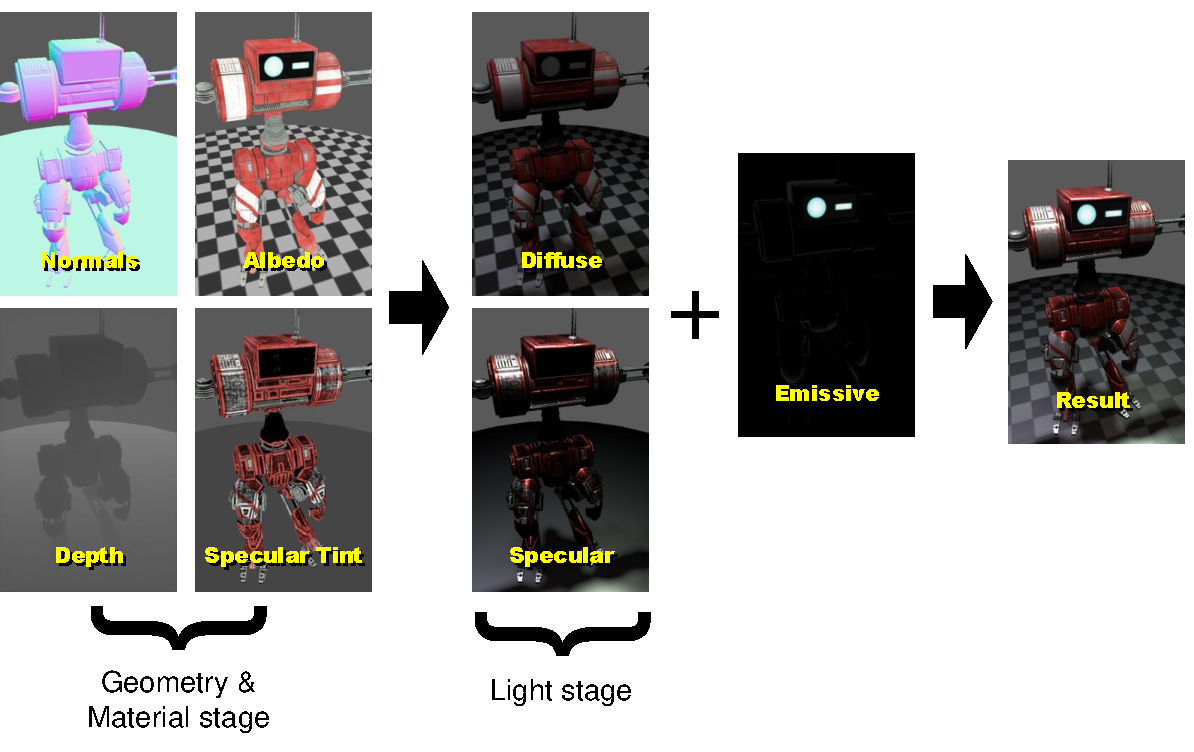
\includegraphics[width=0.9\linewidth]{./Figures/deferredComposition/deferredComposition.pdf}
    \caption[Deferred shading pipeline]{Breakdown of operations in deferred shading. ``UBot'' model courtesy of Eric Andrew.}
  \label{fig:DeferredComposition}
\end{figure}

\item Lights can only influence the scene at the granularity of individual objects, not their vertices or rasterized pixels. Even when a light would affect a small part of an object, it must be evaluated for all elements thereof, because a single \emph{batch} may only use a single shader per domain.

Splitting objects into smaller pieces might be an option, however GPU batch submission carries a nontrivial cost \cite{BatchBatchBatch}, hence the tendency is to do the exact opposite and pack multiple objects into shared batches.
\end{enumerate}

Recently a technique known as \emph{deferred shading} has been gaining popularity, as it offers an elegant solution to both of these problems. Originally proposed in \citet{DeeringDeferred}, the algorithm separates the rendering pipeline into two stages (figure \ref{fig:DeferredComposition}):

\begin{enumerate}
\item Render surface attributes of the visible scene into a set of framebuffers \emph{(collectively called the \textbf{G-buffer})}.
\item For each light, evaluate its contribution on the surfaces encoded within a subset of the \emph{G-buffer}.
\end{enumerate}

Of the two passes, only the first one requires the actual geometry of the scene to be rendered and material shaders evaluated. Similarly, the second pass only runs light shaders. Importantly, each light can be treated separately from another and from material shaders, eliminating the need for merging light and material code -- the main source of the combinatorial explosion of vertex and pixel shaders.

The main strength of deferred shading is at the same time the root of a drawback. Since the second pass only runs light shaders and has no knowledge of the source objects which contributed to the \emph{G-buffer}, it may no longer run per-object shader code. When all objects are just samples in the \emph{G-buffer}, there is no clear way of supporting per-object reflection models.

Another tricky issue is that of translucency. Because the \emph{G-buffer} may only store properties of a single surface at a single fragment location, it doesn't handle translucency in a natural fashion. \citet{HumusDeepDeferred} demonstrates an approach using depth peeling, which is able to overcome this limitation. He uses texture arrays to encode attributes of multiple depth layers. The second pass of deferred shading then computes light influence on each of these layers, stopping on opaque surfaces. This results in good performance for typical scene configurations, since most will have far more opaque elements than translucent ones. The main downside of his approach is the fact that the technique requires $n$ G-buffers in order to support $n$ depth layers, putting much strain on memory.

A more common approach for handling translucency is to render non-opaque surfaces in a separate pass using a traditional forward rendering algorithm. Using read-only depth testing against a depth buffer containing the opaque parts of the scene, translucent surfaces can be blended into the result of deferred shading. A major inconvenience this approach entails is having to maintain both a deferred and a forward renderer, along with material and light shaders which might be used in both of them. The rendering system presented in this work makes it relatively easy by allowing the same \emph{material}, \emph{light}, \emph{reflectance} and \emph{structure} shaders (or \emph{kernels} in its nomenclature) to be used in any of the implemented rendering algorithms.

\subsection{Deferred lighting}
\label{sec:DeferredLighting}

% TODO(?): ref the olde nvidia paper
The regular deferred rendering algorithm requires a large G-buffer, which in some cases may be prohibitive due to memory capacity or bandwidth constraints. \citet{Engel08PrePass} proposes an alternative approach, currently known \emph{light pre-pass}, \emph{deferred lighting} or \emph{pre-lighting}. Unlike classical deferred rendering, which consists of two phases, this algorithm is composed of three stages (figure \ref{fig:LightPrePassComposition}):

\begin{figure}[h!]
  \centering
    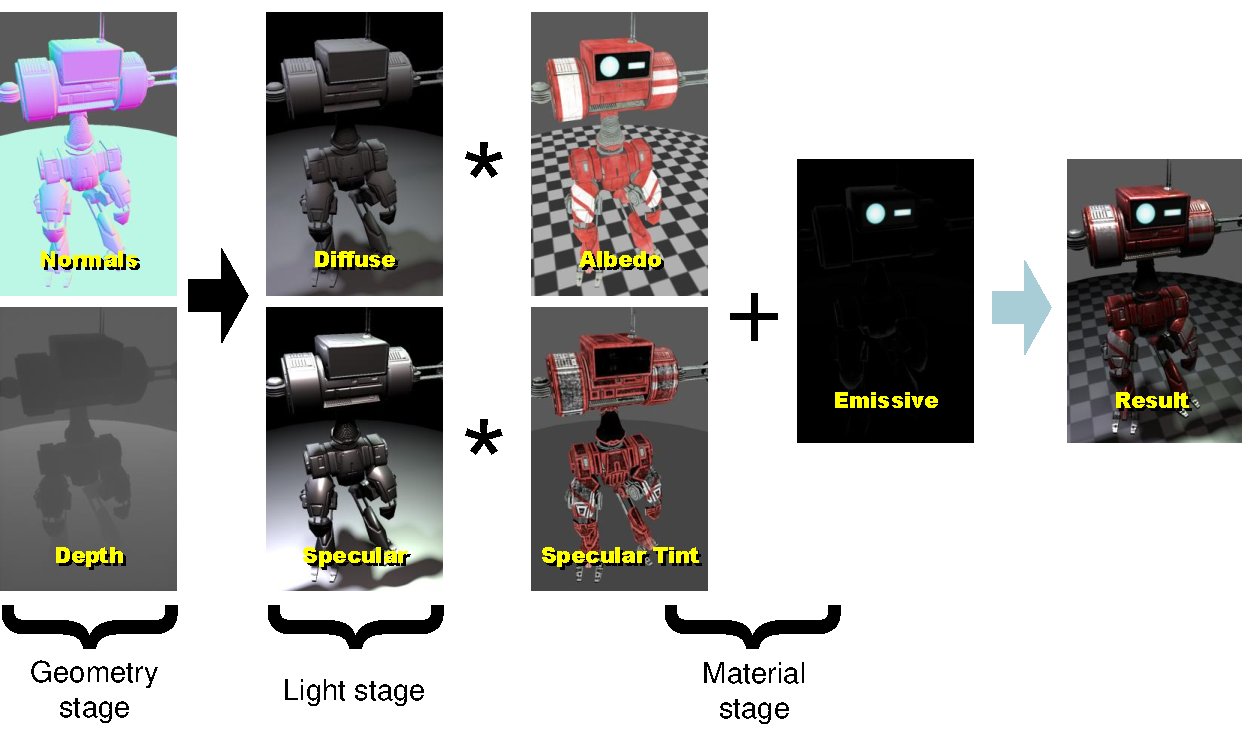
\includegraphics[width=0.9\linewidth]{./Figures/deferredComposition/lightPrePassComposition.pdf}
    \caption[Light pre-pass pipeline]{Breakdown of operations in the light pre-pass rendering algorithm. ``UBot'' model courtesy of Eric Andrew.}
  \label{fig:LightPrePassComposition}
\end{figure}

\begin{enumerate}
\item Render a minimal \emph{G-buffer}, containing the surface depth and normal.
\item For each light, evaluate its contribution on the surfaces encoded within a subset of the \emph{G-buffer} using only the reflectance model.
\item Render scene objects again, this time fully evaluating their materials and combining them with the illumination computed in the previous step.
\end{enumerate}

Such a breakdown of rendering operations trades extra geometric cost for less G-buffer memory utilization, which in particular scene configurations and platforms translates into faster execution.

% http://http.developer.nvidia.com/GPUGems2/gpugems2_chapter09.html

\section{Graph-based systems}

Creating immersive environments requires many complex shaders. \citet{Tatarchuk06ToyShop} mentions that the ``Toy Shop'' demo (shown in figure \ref{fig:ATItoyshop}) contained about 500 custom shaders, so this number can only be expected to be higher in a complete game. It must therefore be easy to create custom shaders, and it must be straightforward for artists in particular.

\begin{figure}[h!]
  \centering
    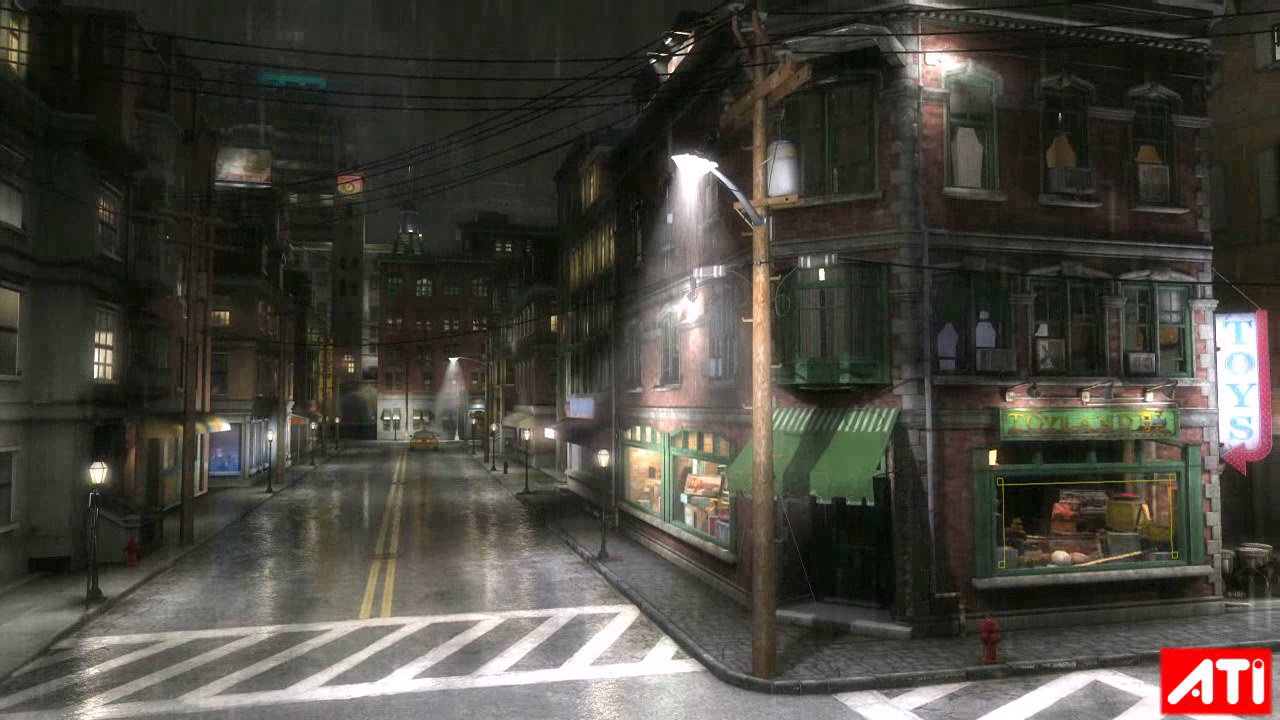
\includegraphics[width=0.9\linewidth]{./Chapters/ati-demo-toyshop.jpg}
    \caption[ToyShop demo]{AMD's real-time Toy Shop demo utilizes about 500 custom shaders. Image courtesy of AMD Graphics Product Group}
  \label{fig:ATItoyshop}
\end{figure}

% http://udn.epicgames.com/Three/MaterialsTutorial.html
% Frostbite, Project Offset, Maya Hypershade, 
A popular approach for enabling artists to easily create shaders is to use a graph-based editor, in which computations and data are represented by nodes. The list of implementations of such systems is getting consistently longer, since despite some shortcomings \cite{ChristerGraphShaderEditorsSuck}, they empower artists to create rich content swiftly, instead of having them rely on programmers for all shaders. This subsequently reduces the communication overhead and takes the load off programmers, resulting in faster product development.

Nevertheless, graph-based shader editors are no silver bullet, do not completely remove the need for efficient communication in a team and must still be designed with care. Simply moving all shader computations into a graph-based representation only turns regular text-based code entry into visual programming, an area which hasn't been adequately explored for production environments.

When \citet{AbramWhitted90} introduced the first visual shader authoring tool, they expressed concern about the possibility of type mis-matches within the data being manipulated by graph-based programs. Indeed, in order to avoid visual clutter, most graph-based tools hide type information of inputs and outputs within nodes. Furthermore, \citet{mcguire2006shadetrees} points out that this mis-matching issue extrapolates onto semantic meaning of data:
	
\begin{quote}
In fact, this problem extends beyond storage types to interface mismatches between atoms, e.g., assumptions like “the light vector has unit length” or “RGB values are pre-multiplied by the alpha channel.” It is almost impossible for the user to ensure that the types are correct when the programming tool conceals those types. 
\end{quote}

In a summary, a graph-based shader authoring tool should not be implemented in a naïve manner. Doing so means that neither artists nor programmers are able to use it effectively. Another important point to note is that if a graph-based shader authoring tool only allowed, for instance, direct pixel shader editing, then the vertex shader would need to be kept in sync in some way. Hence the second goal besides solving type mis-match issues is a paradigm shift, one which frees the artists from the subdivision imposed by the GPU architecture.

One example of a renderer which decouples artists from thinking in terms of vertex and pixel shaders is \emph{Frostbite}. In \cite{AT07}, Andersson details that their approach uses graph-based \emph{surface} shaders. Similarly to the ones in \emph{RenderMan}, they decouple material properties from lighting, environment and geometry. All shaders are treated as content instead of code, and as a part of the pipeline, converted to an efficient representation for run-time processing. The \emph{Frostbite} engine has to date been used in a few large games, running on the PC, Xbox and PS3 platforms, being a testament to the practicality of the solution.

\subsection{Abstract Shade Trees}

\citet{mcguire2006shadetrees} introduce \emph{Abstract Shade Trees} which tackle the type mismatch problem \cite{AbramWhitted90} in an interesting manner. The key concept their paper introduces is embedding \emph{semantic} information in types used to define the interfaces of computational atoms. They subsequently use a \emph{weaver} algorithm to automatically connect atoms and perform type coercions.

They note that regular types used by a shading language such as GLSL are "merely C-style storage specifiers with little value as abstractions. For example, a color, a 3D location, and a row of a 3×3 matrix have the same type, which is also indistinguishable from an array of three floating-point numbers." On the other hand, their \emph{semantic types} are able to carry more meaningful information, such as:
\begin{itemize}
\item The \textbf{Basis} in which instances of this type are defined (tangent, object, world, screen).
\item \textbf{Length} of a vector (unit, any).
\item The very interpretation, e.g. whether it's a color, a texture coordinate or a normal vector.
\end{itemize}

Such a type system allows stronger checking, but it also enables automating tedious tasks such as coordinate-space conversions. For example, when one atom outputs a position vector in \emph{object} space, and another requires the position in \emph{world} space, it becomes possible to generate code to perform the required math.

\begin{figure}[h!]
  \centering
    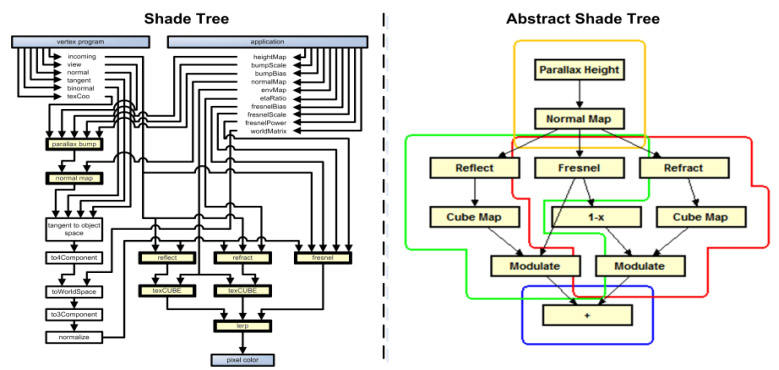
\includegraphics[width=0.9\linewidth]{./Chapters/AbstractShadeTree.jpg}
    \caption[Abstract Shade Tree]{A conventional Shade Tree (left) and the equivalent Abstract Shade Tree (right). Image courtesy of McGuire et al.}
  \label{fig:AbstractShadeTree}
\end{figure}

An \emph{Abstract Shade Tree} is normally much more compact than an equivalent \emph{conventional Shade Tree}, as demonstrated by Figure \ref{fig:AbstractShadeTree}. Thanks to the complexity hiding, shader authoring becomes less error prone and especially easier for users who do not have knowledge of programming concepts such as types, variables or the vector math used to implement algorithms inside atoms.
 
The rendering system presented in this work utilizes a \emph{semantic type system}. In contrast to Abstract Shade Trees, automatic determination of fine-grained dependencies between atoms is not central to its function. Manual connections of inputs and outputs are allowed in addition to setting coarse-grained dependencies. Both the former and the latter are then subject to automatic type coercions, hence type safety is retained. The work of McGuire et al. is also extended by the introduction of \emph{semantic expressions}, which provide parametric polymorphism and basic type algebra for atom parameters.
